% !TeX program = lualatex

\documentclass[12pt]{report}

\usepackage{url}
\usepackage{hyperref}

\usepackage{graphicx} % images
\usepackage{subcaption}

\usepackage{fontspec}
\setmainfont{Times New Roman}

\linespread{1.25} % the equivalent of 1.5 line spacing from msword

% margins
\usepackage[a4paper, left=2.5cm,right=2.5cm,top=2.5cm,bottom=2.5cm]{geometry} 

\usepackage{amsmath}

\usepackage[]{algorithm2e}

\usepackage{todonotes}
\usepackage{wrapfig}
\usepackage{afterpage} % image positioning

\usepackage[utf8]{inputenc} % romanian characters

\usepackage[numbers]{natbib}

\begin{document}
	\pagenumbering{gobble}% Remove page numbers (and reset to 1)
	
	\begin{titlepage}
		
		\begin{center}
			\Large{{UNIVERSITATEA BABEȘ-BOLYAI CLUJ-NAPOCA}}
			\Large{{FACULTATEA DE MATEMATICĂ ȘI INFORMATICĂ}}
			
			\vspace{4cm}
			
			\textbf{LUCRARE DE DIPLOMĂ}
			
			\vspace{1cm}
			\Huge\textbf{{O ABORDARE HIBRIDĂ BAZATĂ PE CARACTERSISTICI DE CULOARE ȘI TEXTURĂ PENTRU SEGMENTAREA PIELII UMANE ÎN IMAGINI}}
			\fontsize{12}{14}
			
		\end{center}
		\vspace{6cm}
		
		\hspace*{0.8cm}Coordonator  Științific: \hfill  Absolvent: \hspace*{0.8cm} \\    
		\textbf{Dr. Mircea Ioan-Gabriel, Asistent Universitar \hfill  \textbf{Ștefan Sebastian}}
		
		\vspace{2cm}
		\begin{center}
			\Large{2018}
		\end{center}
	\end{titlepage}
	
	\begin{titlepage}
		
		\begin{center}
			\Large{{BABEȘ-BOLYAI UNIVERSITY CLUJ-NAPOCA}}
			\newline
			\Large{{FACULTY OF MATHEMATICS AND COMPUTER SCIENCE}}
			
			\vspace{4cm}
			
			\textbf{DIPLOMA THESIS}
			
			\vspace{1cm}
			\Huge\textbf{{A HYBRID APPROACH BASED ON COLOR AND TEXTURE FEATURES FOR HUMAN SKIN SEGMENTATION}}
			\fontsize{12}{14}
			
		\end{center}
		\vspace{6cm}
		
		\hspace*{0.8cm}Supervisor: \hfill  Author: \hspace*{0.8cm} \\    
		\textbf{Dr. Mircea Ioan-Gabriel, Assistant \hfill  \textbf{Ștefan Sebastian}}
		
		\vspace{2cm}
		\begin{center}
			\Large{2018}
		\end{center}
	\end{titlepage}

	\cleardoublepage
	ABSTRACT
	\vspace{0.5cm}	
	\hrule
	\vspace{0.5cm}	
	
	The subject of this thesis is the problem of human skin detection in images. The goals are to provide an analysis of the current state of research in this area, present the theoretical foundations required to build a skin detector and to propose a new model, focused on reducing the false detection rate.
	
	With the current evolution in computing power, a lot of complex image analysis tasks are now viable for consumer devices. These include human computer interaction systems such as face detection, hand sign recognition or gesture analysis, monitoring systems and data mining for human related features. Most of these types of systems use skin detection as a preprocessing step, because the presence and shape of skin provide a good indication of the presence or location of a person. Consequently there is a need for fast and accurate human skin models.
	
	This paper proposes an algorithm that aims to improve the high false acceptance rate typical of skin detectors found in research. The motivation behind this is that most skin detectors focus on computation speed rather than performance. Consequently there is a lack of accurate skin models for tasks where computation speed is not crucial, such as data mining.
	
	The proposed model is a hybrid of already proven techniques. It analyzes color information on regions detected through image segmentation and then applies a texture filter to further reduce false acceptance rate. Images are segmented using the Quick shift algorithm which takes into account pixel color and position features. For each of the resulting superpixels an average skin probability is computed using Skin Probability Maps. Haralick's textural features are calculated on a window around each pixel and classified with a Support Vector Machine. Finally, the results of the color and texture models are intersected. 
	
	The model achieves similar results to state-of-the-art detectors but it does not fulfill the goal of severely reducing false acceptance rate. However, the results are not conclusive because evaluation was done on a smaller dataset due to time constraints.
	
	To my best knowledge, a skin detection model using image segmentation, color and texture information has not yet been published in this area of research. This work is the result of my own activity. I have neither given nor received unauthorized assistance on this work.
	
	
	\tableofcontents
	\listoffigures
	\listoftables
	\newpage
	
	\pagenumbering{arabic}
	
	\chapter{Introduction}
	
	This chapter introduces the topic of skin detection with its applications, the motivation behind the proposed model, alongside an overview of its main components, and the outline of the following chapters.
	
	The problem tackled in this paper is skin detection in images. Skin detection, as a field of research,  means identifying pixels and regions in images which correspond to human skin. The goal of skin identification is usually to build a more complex model, like a face or hand gesture detector.
	
	The problem statement is a simple one however its application comes with a lot of challenges such as: various illumination conditions, multiple possible skin colors, presence of objects that resemble skin.
	
	\section{Applications of skin detection}
	
	\subsection{Pornography filtering}
	It is a known fact that internet has become a commodity of modern life, with an average global penetration rate of 54.4\% \cite{internet_stats}. This means that it's inevitable for a large number of children to have unrestricted access to the internet and to be exposed to harmful content. A study conducted in England \cite{children_exposure} on over a thousand people aged 11-16 has revealed that over half of them have been exposed to pornographic content. 
	
	To avoid such scenarios various pornography filters have been created. Skin detection is a very useful step in implementing such an application because most pornographic images contain large areas of skin.
	
	One approach is described by Fleck et al. \cite{finding_naked_people}. The model proposed in that paper scans the images for large areas of skin and then applies some geometrical analysis looking for elongated shapes. This model was tested using 138 images of naked people and 1401 assorted images, some containing people but not naked. The system obtained a 52\% recall and 60\% precision against a large control set (1401 images).
	
	Another similar approach was presented by Chan et al. \cite{pornography_filter_with_ratios}. The first step was skin extraction based on color which was followed by computing some high level features such as: the ratio of skin area to image area, the ratio of the largest skin segment to the image area and the number of skin segments in the image.
	
	\subsection{Anchorperson detection}
	Another application that was created in practice is anchorperson detection in talk shows  \cite{anchor_person_detection} for automatic annotation and storage. The data can be used for quickly finding videos containing specific persons, calculating how much time each anchorman was on stage or other data mining tasks. This is an ideal application for skin detection because news videos are usually shot indoors in a controlled environment. Consequently, the background can be set up so it won't contain objects with skin color tones.
	
	\subsection{Preprocessing for complex systems}
	While skin detection does not have many direct applications, it is usually an intermediary step for detecting more concrete body parts, so I will also present some applications of those methods.
	
	Face and hands detection is used to facilitate human computer interaction. By scanning gestures and reactions a software system can respond in a more convenient way to the user. For example the Kinect camera, which connects to the Xbox console, allows the user to navigate menus using hand swipes \cite{kinect_control}. 
	
	Aside from convenience gesture recognition systems can be very helpful for people that are aging or recovering after an accident or disease. Applications such as the one presented by Pedraza-Hueso et al. \cite{rehabilitation_kinect}, are designed to help these types of people get into a better physical shape. Typically they run on a video console like Kinect or Wii and take the form of games. These consoles make the users stand-up and perform different types of motions while playing. The main advantages of using such an application are: availability (users can do their exercises at any time in their own home), price (typically much lower than hiring a therapist) and entertainment (applications usually take the form of games which stimulate the user).
	
	Face recognition, the next step after detection, means automatic identification of people in images or videos \cite{detecting_faces_a_survey}. This has applications in security, such as unlocking your phone only when it scans your face, and monitoring certain areas, like the systems used by the Chinese government to fine jaywalkers caught on camera without human intervention \cite{jaywalkers_china}. A trivial yet very popular use of face recognition is automatically tagging your friends in photos on social networks.
	
	\section{Motivation}
	As a consequence of all the difficulties of building an accurate skin model, briefly noted at the beginning of the chapter, and the fact that most use cases of skin detection need real time response times, most skin detectors use only the color features and have a rather high false positive rate, of over 10\% \cite{survey_skin_color_modeling}. 
	
	This paper proposes a new model that focuses on classification performance rather than computation speed in the attempt to reduce the false positive rate. In this regard, the method described in this paper tries to combine multiple state-of-the-art techniques to determine if it can obtain a more accurate detector than the classical color-based approaches. This would also fill a gap of skin detectors oriented for analysis tasks, that don't rely on real time responses.
	
	\section{Solution overview}
	The model presented in this paper is a combination of three proven skin detection techniques, concerning image segmentation, color analysis and texture filters. The personal contribution is given by combining these techniques into an unified model and examining its behavior.
	
	First of all, the input image is segmented using the Quick shift algorithm. The result of this step is a list of regions that are homogeneous in shape and color avoiding the issue of having holes in skin-like regions. These blocks have their color analyzed using Skin Probability Maps that rely on Bayes' Theorem, a classical approach that identifies most skin-colored regions. However, this means using a naive Bayes classifier, because it relies on the assumption that color is the only relevant feature. 
	
	To further reduce false acceptance rate, a texture analysis module is used. Haralick's statistical features are computed on a window around each pixel of the image and passed into a Support Vector Machine classifier. The pixels marked by both the color and the texture models are used to build the final skin mask.
	
	\section{Thesis outline}
	Next, the main chapters along with a brief overview will be presented.
	
	\textbf{The second chapter} focuses on the theoretical background of the subject. It starts with the presentation of the problem statement which is followed by a list of state-of-the-art solutions found in literature. This related work section is organized by the main approach used in the papers. Afterwards a theoretical overview of the main solution modules is given in the following order: image segmentation, skin color analysis, texture detection.
	
	\textbf{Chapter 3} gives a detailed presentation of the model proposed by this paper. It is focused on the particular choices taken while building it, such as the selected parameters and feature extraction functions, rather than the underlying theory which is explained in the second chapter. Next, training and evaluation methodologies and the datasets used for each are described. The model's results are presented at the end of the chapter, alongside a comparison with other approaches found in literature.
	
	\textbf{Chapter 4} focuses on the concrete implementation of the proposed model. It contains all details related to technologies used and application design. The first section
	provides a brief introduction for all frameworks and libraries used in this project. The following section presents the breakdown of the program into modules and the implementation decisions for each of them, alongside a general view given by use case and sequence diagrams. The last section provides a user manual which describes the application's functionalities in depth.
	
	\textbf{The last chapter} contains the conclusions. It presents the current state of research in skin detection, a short evaluation of the proposed model and proposals for future improvements to it.
	
	\chapter{Theoretical background}
	This chapter provides the theoretical background necessary for creating a skin detector. It starts with an introduction of the topic and its challenges. This is followed by a review of the best-performing models available in research. Afterwards, the next three sections introduce the theoretical concepts on which the proposed model relies.
	
	Skin detection in images is the problem of identifying pixels or regions in an image that correspond to human skin. This is most often a preprocessing step for more complex detectors of specific body parts. Some of these applications are created for data-mining and require more precise answers while other try to provide real-time detection which means it is imperative to have fast response times. This means the model designer should take into account the specific area in which it will be used and consider the trade-off between speed and accuracy.
	
	In order to obtain a skin model some features need to be computed. The most reliable and widely adopted is the skin color. Models built on this feature are the most popular because of their speed and robustness to scaling and rotation \cite{survey_skin_color_modeling}. Texture is another useful feature that can describe skin. However, the fact that skin does not have a very distinct textural pattern means that a texture classifier alone is usually not enough. Shape could be another feature, however it is rarely used in practice because skin patches can have irregular forms.
	
	Although the problem statement is quite simple and doesn't require a lot of domain knowledge, the practical applications have a lot of challenges to overcome. A good skin detector should provide solutions for the issues presented next \cite{survey_skin_color_modeling}. First of all, one of the most challenging aspects is handling illumination. While the human eye can easily distinguish the same color in varying degrees of brightness this is not a trivial task for computers. The second aspect to be considered is the variety of skin tones. A good model should be able to handle people of all races. Another thing to note is the fact that there are a lot of objects and materials that resemble skin such as leather, wood, sand etc. Consequently, most models have a rather large false positive rate (over 10\%).
	
	\section{Related work}
	The subject of skin detection has been of interest for researchers due to its many applications. I could not include all the important papers in this domain due to the sheer number but I tried to cover the most relevant ones, in terms of popularity and results, for each aspect of skin detection.
	
	\subsection{Models using color analysis}
	
	\subsubsection{Skin Probability Maps}
	One of the most comprehensive experiments in skin detection was conducted by MJ Jones and JM Rehg \cite{compaq} who created the Compaq skin dataset, which became a standard for evaluating results of research in this domain. Their main approach was building a Skin Probability Map based on Bayes' Theorem. The resulting classifier, published in 1998, has obtained results comparable to modern approaches.
	
	Skin probability maps are histogram based models, meaning they set a number of bins for each color channel where they keep track of how many times each color pixel appears in the training set. Although \(256^3\) would be an obvious choice for the number of bins (one for each pixel value) they determined that \(32^3\) is the optimal value.
	
	Jones and Rehg \cite{compaq} made the observation that given even a large training set most pixels are never seen. They explored their dataset of approximatively 2 billion pixels and came to the conclusion that around 77\% of the RGB space is empty. This comes in support of their decision to use larger bins, like \(32^3\).
	
	For this model they used a 6822 photo training set, where 4483 photos contained no skin and 2336 had portions of skin. The testing set had similar dimensions: 6818 total photos (4482 non-skin and 2336 skin). Using these methods they obtained a 80\% true positive rate and 8.5\% false positive rate or, with a different threshold, a 90\% TP rate and 14.2\% FP rate.
	
	\subsubsection{Gaussian Models}
	This approach consists of modeling human skin distribution as a Gaussian probability density function or a combination of Gaussian functions.
	
	The previous paper \cite{compaq} by Jones and Rehg also proposes a combination of two mixture models for skin and non-skin classes. Each model is composed of 16 gaussians and was trained on approximatively 74\% of the histogram data, because only that data was available at the time. The results were similar to those of the previous model: 80\%/9.5\% and 90\%/15.5\%.
	
	Lee and Yoo \cite{gaussian_applied} implemented a Single Gaussian in CbCr and a Gaussian Mixture in IQ, both trained and tested on the Compaq dataset with the results of 90\%/33.3\% and 90\%/30\%, respectively.
	
	Yang and Ahuja \cite{Yang99gaussianmixture} proposed a finite Gaussian mixture model. They theorized that this offers an improvement over a single Gaussian function and justified this hypothesis using statistical tests on normality and number of components, namely the Hawkins' Test on Normality and Homoscedasticity and McLachlan's Bootstrap Test. The selected method of determining the model's input parameters is the Expectation Maximization (EM) technique. This experiment was performed on the Michigan face database that contains aroung 9.5 million skin pixels. The pixels were transformed from RGB to CIE LUV color space in order to separate and then remove the illumination component. The next step was applying a segmentation algorithm on the image and then analyzing each pixel's color. Every region that had more than 70\% of its pixels classified as skin was labeled as a skin region. However, they did not offer and performance metrics on their experiment.
	
	\subsubsection{Elliptical boundary model}
	This is a statistical model proposed by Lee and Yoo \cite{gaussian_applied} as an alternative to Gaussian models. The limitations that this model tries to overcome are the single Gaussian's luminance sensitivity and the mixture's slow training speed.
	
	This model relies on the observation \cite{Yang99gaussianmixture} that in most color spaces skin pixels tend to form an ellipsoidal cluster. The training algorithm has two steps: preprocessing and parameter estimation. The first step removes outliers in order to focus on the underlying density of the data set. This consists in removing the first k\% samples with the lowest frequency. k is usually chosen in the 0 to 5 range.
	
	The elliptical boundary model is defined as $ \Phi(X) = [X - \Psi]^T\cdot \Lambda^{-1} \cdot [X - \Psi]  $ where X is the chrominance vector of the considere pixel. $\Psi$ is the average value of skin pixels in the training set. $\Lambda$ is calculated as $ \frac{1}{N} \cdot \sum_{i=1}^{n}f_i(X_i-\mu)(X_i-\mu)^T$ where $\mu$ is the mean of chrominance vectors and $f_i$ their number of apparitions in training. T represents the model's threshold.
	
	This model obtains an average of 90\% TP rate and 23.3\% FP rate on the Compaq dataset.
	
	\subsubsection{Explicit thresholding}
	Another popular approach is explicit thresholding. This domain consists of finding simple rules that apply to each pixel's color features and determine based on their results if the considered pixel is part of the skin class. Some examples include \cite{rgb_threshold}, \cite{cr_cb_threshold}, \cite{yiq_threshold}, \cite{i_threshold} for face detection systems in different color spaces with varying results. 
 	
 	A set of thresholds for YCrCb space where proposed by Chai and Ngan \cite{cr_cb_threshold}. They set the ranges for Cb from 77 to 127 and for Cr from 133 to 173 and worked with the ECU database.
 	
 	Dai and Nakano \cite{yiq_threshold} created a model for YIQ, an orthogonal color space, which only used the I component (which stands for in-phase). The range they provided was [0, 50], however most of the images in their databases where of people with yellow skin.
 	
 	Brand and Mason \cite{i_threshold_applied} applied the technique from Wang and Brandstein's paper \cite{i_threshold}, which uses the YI'Q' space with the following threshold \(14 < I' < 40\), on the Compaq dataset and obtained 94.7\% TP rate and 30.2\% FP rate.
 	
 	An interesting approach, proposed by Gomez and Morales \cite{rca_threshold}, is having a learner find these rules. They use RCA, a constructive induction algorithm, to build rules expressed with simple arithmetic operations in the rgb space. Their method achieves better results than the Bayesian SPM on their dataset, however it is computationally slower. RCA stands for Restricted Covering Algorithm which resembles a general covering algorithm with the restriction of trying to build a single rule for each class (in this case, a rule for skin detection). The strategy implemented for RCA was finding attributes which cover either a large number of true positives or a few false positives. The starting attributes where r, g, b and the constant 1/3, which would generate new attributes using the operators : +, *, - and squaring. One of their best and simplest generated models looks like this:
 	\begin{equation}
 	\begin{split}
 	\frac{r}{g} > 1.185 \quad \textrm{and}\\
 	\frac{r * b}{(r + g + b)^2} > 0.107 \quad \textrm{and}\\
 	\frac{r * g}{(r + g + b)^2} > 0.112
 	\end{split}
 	\end{equation}
 	In comparison with the C4.5 decision tree algorithm, the RCA method obtained slightly worse results but with much simpler rules. They used a custom dataset containing images of more than 2000 people and obtained around 90\% both in precision and recall.
 	
 	\subsubsection{Hidden Markov Models}
 	Sigal et al. \cite{hmm} implemented a method for real time skin detection in videos. Their model predicts the evolution of the skin color histogram using a second order Markov model, with an initial prediction from a Bayes classifier over the Compaq dataset. It uses the EM algorithm which consists of two steps: E(frame segmentation based on histogram) and M(histogram adaptation based on feedback from the current frame).
 	
 	\subsection{Models using segmentation}
 	Frerk and Al-Hamadi \cite{superpixels_applied_1} proposed a method that applies image segmentation combined with a Bayesian SPM. The first step is calculating the skin probability for each pixel in an image and creating \(P_I\), the pixel probability image. The color and position of each pixel is used as input for a SLIC algorithm, an adaptation of k-means, that calculates the superpixels. The parameter k for segmentation is set to be the number of pixels in the image divided by \(30^2\), so that all regions have a size of approximatively 30x30. A probability is then computed for each superpixel and compared to a threshold.
 	
 	Poudel et al. \cite{superpixels_applied_2} took a similar approach to Frerk and Al-Hamadi's \cite{superpixels_applied_1} work. Firstly, a segmentation is performed (using the Quick shift algorithm) and superpixels are extracted. A probability is calculated for each superpixel as the average of its component pixels probabilities. Then, a CRF(Conditional Random Field) method is used in order to obtain smoother skin regions. A CRF is a probabilistic method that works with graph based structures and models a distribution of type $P(y|x)$. The pair considered in this article is color difference and boundary length between neighboring superpixels. This model was tested on the Compaq database and obtained a 91.17\% TP rate and 13.12\% FP rate.
 	
 	\subsection{Models using textural features}
 	
 	\subsubsection{Haralick features}
 	El Abbadi et al. \cite{color_texture_ann} presented a model based on Artificial Neural Networks that analyzes both color and textural features. The color features used are the mean color, the standard deviation and the skewness. These are calculated for each channel (R, G, B). The inputs for the ANN also include the following textural information: Entropy, Energy, Contrast and Homogeneity, which are computed from the Gray-Level Co-Occurrence Matrix. The network has three layers: an input layer, a hidden layer (with 50 neurons) and an output layer. The model was trained on 300 images (80x80 px) of skin and non-skin textures and tested on 100, obtaining a 96\% accuracy in classifying whether an image is a skin patch or not.
 	
 	Medjram et al. \cite{texture_svm} proposed another method that combines color and texture information. The first step is converting the initial image to the YCbCr color space. Skin regions are identified using thresholding like the following: \(77 <= Cb <= 127, 133 <= Cr <= 173\). Next, the image is sharpened in order to enhance its texture. The features considered from the GLCM are Contrast, Homogeneity and Energy, calculated over a 5x5 matrix. The last step is applying a Support Vector Machine classifier on the initial image to classify texture patches. They do not provide any performance metrics only a remark that the model performs well after being tested on hundreds of internet images.
 	
 	\subsubsection{Gabor wavelet transforms}
 	Jian, Yao et. al. \cite{texture_gabor_wavelet} use Gabor wavelet transforms to compute textural attributes. This step comes after an initial skin probability map calculation with the aim of reducing its false acceptance rate. 
 	
 	Gabor transforms are filters that analyze orientation and frequency using complex sinusoidal functions. Before applying this filter the image is converted from RGB to grayscale using the following equation $I(x,y)=0.3R(x,y)+0.59G(x,y)+0.11B(x,y)$.
 	
 	To evaluate this model they used their own manually labeled data set of 600 images. A simple SPM approach got 92.7\%/20.1\% TPR/FPR while the proposed method obtained 94.8\%/4.2\%.
 	
 	\subsubsection{Contourlet-Based Analysis}
 	Fotouhi et al. \cite{contourlet_texture} proposed a model that uses texture segmentation based on nonsubsampled contourlet coefficients. 
 	
 	A first step is using boosting to predict the class of each pixel using its color features. For this approach several Gaussian mixture models are chosen for the $YC_rC_b$, normalized rgb and HSV color spaces. This obtains a 93.1\% TPR and a 22.8\% FPR.
 	
 	Next, a contourlet transform is applied over the whole image. For each pixel that was classified as skin by the previous method a 8x8 patch is selected in each subimage. These vectors are concatenated with the Principal Component Analysis technique and then fed into a Multilayer Perceptron for classification. The final model obtains a 82.8\%/7.6\% TPR/FPR rate.
 	
 	\subsection{Models using shape information}
 	This approach is usually applied for the detection of specific skin regions such as faces \cite{face_detection_shape} or hands \cite{hand_detection_shape} which have predefined and easy to identify shapes. However, there are some general skin detectors that consider shape features. They are based on the assumption that most skin patches, like faces, hands or legs, have an elliptical shape.
 	
 	Such a model was proposed by Kruppa et al. \cite{skin_detection_shape}. Their approach works in two steps. Similar to other FAR reducing techniques, the first step is applying a skin color detector as it provides a good starting point for further refinement. After identifying skin color regions a skin patch filter is applied that finds elliptical shapes in the image.
 	
 	\begin{equation} \label{shape}
 	S(x_c, y_c, w, h) =  \left\{
 	\begin{array}{ll}
 	\frac{1}{1+exp^{-a}} & if \quad \frac{(x-x_c)^2}{w^2} \pm \frac{(y-y_c)^2}{h^2} \le 1\\
 	0 & else \\
 	\end{array} 
 	\right. 
 	\end{equation}
 	
 	The shape model can be seen in figure \ref{shape}. In this equation $(x_c,y_c)$ denote the center and w, h the dimensions of the ellipse and a is a parameter used to smooth out probabilities. These parameters are derived from the skin color model using a technique to maximize mutual information between two probabilities.
 	
 	This model was tested on a data set of 653 images resized to 150x100 resolution. The authors report an improvement over the classical color model by up to 25\% in the error rate value.
 
 	\clearpage
	\section{Image segmentation}
	Image segmentation is a technique for dividing an image into several regions that contain similar pixels. These partitions are often called super-pixels and represent an abstraction layer over the initial image. They can be characterized by color, border or shape(circle, ellipse, polygon, etc.) \cite{computer_vision_book}. The main purpose of segmentation is to represent areas of interest in an image such as faces, fields, buildings, etc, and usually serves as a preparation step for a more complex detection algorithm.
	
	Ideally, the resulting regions should have the following characteristics: uniformity according to the selected feature, such as color or texture, a small number of holes(subregions that differ considerably from the container region), a notable difference from the neighboring areas and smooth borders. \cite{computer_vision_book}.
	
	This problem has been researched extensively over the years however there is not a single best solution available. I will present some of the algorithms presented in literature.
	
	\subsection{Thresholding}
	Thresholding is one of the simplest approaches to image segmentation. It consists of finding a threshold T for the gray level of pixels in the image. Therefore, we can classify every pixel by comparing its brightness to T. This technique is a perfect fit for separating objects from a darker background but has severe limitations in other tasks \cite{image_segmentation_techniques}.
	
	One of the problems with global thresholding, choosing a single value for T over the whole image, is dealing with different levels of illumination. For that reason the local thresholding approach was developed. This expands the previous method by using multiple thresholds for different parts of the image. Chow and Kaneko  \cite{segmentation_thresh_multiple} applied a similar method for detecting the left ventricle of the heart in x-ray pictures. They divide the original image in multiple blocks that do not overlap and calculate a threshold for each of them.
	
	Threshold selection can be done manually or automatically and usually involves analysis of a gray level histogram where the size of each bar is proportional to the number of pixels with that brightness \cite{review_on_image_segm_tech}. For example, in an image that contains some objects in front of a darker background the histogram is likely to contain two peaks separated by a valley and we can choose T somewhere in between those peaks. 
	
	Automatic threshold detection can be done by modeling object and background populations with a normal distribution like the experiments presented in  \cite{experiments_on_thresholding}. The method proposed calculates a least-squares fit of a function f(i), where i is the gray level, to the histogram, using a hill climbing algorithm. The function takes into account the mean and standard deviation of the histogram. Lastly, the best fitting f(i) is the used for classification.
	
	However simple, all these methods have limitations, such as not considering spatial factors, and having no control over border smoothness and holes inside detected regions.
	
	\subsection{Edge detection}
	These methods aim to solve image segmentation problems by detecting all edges in images. An edge is characterized by a sudden change in pixel intensity \cite{image_segmentation_techniques}. The result of edge detection is an image that represents to classes of pixels: part of an edge or not. I will present some of the most popular methods.
	
	The Roberts Detection \cite{edge_detection_survey} is one of the fastest methods due to its simplicity. It uses the following convolution masks:
	\[
	Gx =
	\begin{bmatrix}
		1 & 0 \\
		0 & -1 \\
	\end{bmatrix}
	Gy =
	\begin{bmatrix}
	1 & 1 \\
	-1 & 0 \\
	\end{bmatrix}
	\]
	Each of theses calculates a gradient value for an orientation and their values can be combined to determine an absolute magnitude of the gradient using: \(|G|=\sqrt{G_x^2 + G_y^2}\). Lastly, we can apply thresholding for the resulting value to determine if it is part of an edge or not.
	
	Other similar detectors are the Prewitt and the Sobel detectors \cite{edge_detection_survey}. The difference is that they use a larger convolutional mask, 3x3, and in case of the former, more orientations.
	
	Some soft computing techniques such as: neural networks, genetic algorithms and fuzzy logic \cite{edge_detection_survey}, have also been applied in edge detection problems. However they don't offer significant improvements in performance over the simpler and faster methods.
	
	\subsection{Clustering}
	We can view the image segmentation process as a clustering problem. All pixels are associated with a region, which corresponds to a cluster.
	
	\subsubsection{K-means}
	One popular approach to segmentation problems is the K-means algorithm, which can divide n data points in k clusters, where k is known in advance. This can be applied to image segmentation if we consider pixel intensities as the values on which we are doing clustering. The algorithm is simple and efficient on large volumes of data \cite{image_segmentation_techniques}, however the number of clusters must be known in advance, which can be problematic as the number of distinct regions can vary from image to image.
	
	\subsubsection{Mode seeking. The Quick shift algorithm}
	Mode seeking algorithms are methods for clustering without needing to know the number of clusters in advance. The first step of these algorithms, as presented in  \cite{mode_seeking}, is calculating a Parzen density estimate over all given points: \(P(x)=\frac{1}{N} \cdot \sum_{i=1}^{N} \cdot k(x-x_i)\). The next step is moving each point towards a mode of P(x) on a trajectory determined by the gradient of P. Clusters are formed by the points converging on the same modes.
	
	The Quick shift algorithm \cite{quickshift_gpu} is one of the most efficient in this family. It starts by calculating a Parzen density estimate, most often using an isotropic Gaussian window:
	\begin{equation}
	P(x) = \frac{1}{2 \pi \sigma^2 N} \cdot \sum_{i=1}^{N} e^\frac{-\Vert x - x_i \Vert^2}{2 \sigma^2}
	\end{equation}
	Every point is then linked to the nearest one with a higher density and the resulting structure is a tree. In order to get our regions we can either cut branches with a size larger than \(\tau\) or analyze data points less then \(\tau\) distance away on the linking step. If we choose the latter, the result will be a collection of trees, each representing a cluster.
	
	In the application of Quick shift in image segmentation a relevant feature space must be chosen. An option is using the RGB components and position(x, y coordinates) of each pixel. As the position does not always have fixed bounds (image size can vary) we can scale the position components depending on our input data, such that the importance of color and position remains similar\cite{quickshift_gpu}.
	
	An example pseudocode implementation as presented in \cite{quickshift_gpu} can be seen in figure \ref{alg:quick_shift}.
	
	\begin{algorithm}
		\caption{The Quick shift segmentation algorithm}
		\label{alg:quick_shift}
		\# density computation\;
		\For{x in all pixels}{
			P[x] = 0\;
			\For{n in all pixels less than 3 * $\sigma$ away}{
				P[x] += exp(-(f[x] - f[n])\^{}2 / (2 * $\sigma$ * $\sigma$))	
			}
		}
		\# neighbor linking\;
		\For{x in all pixels}{
			\For{n in all pixels less than $\tau$ away}{
				\If{P[n] \(>\) P[x] and distance(x, n) is smaller than to previous parent}{
					d[x] = distance(x, n)\;
					parent[x] = n\;
				}
			}
		}
	\end{algorithm}
	When calculating the density we limit our search to a 3$\sigma$ window because the contributions for pixels further away should be small \cite{quickshift_gpu}.
	
	Some advantages of Quick shift are simplicity of implementation, speed (O($N^2$)), ability to work on any type of data and the control of fragmentation with the given parameters \cite{mode_seeking}. 

	\clearpage	
	\section{Skin detection by color}
	Skin pixel detection by color means classifying a pixel while considering only its color features. A first step in applying this approach is selecting a color space.
	
	\subsection{Color spaces}
	A color space, also called a gamut, represents a set of colors in a way that is independent of the medium in which they are represented(computer screens, cameras, magazines, etc) \cite{color_management_guide}. The L*a*b* color space contains all colors that can be seen by the human eye, however most color spaces are smaller due to technical limitations. I will present some of the color spaces which have been used successfully to classify skin pixels. 
	
	\subsubsection{RGB}
	To start with, RGB is one of the most popular color spaces for working with image data. It matches the color sensitive receptors of the human eye(red, green, blue) and started as a convenient way to represent the colored rays used by CRT screens \cite{survey_color_detection_techniques}. While this model is simple to use it has the disadvantage of mixing chrominance and luminance features \cite{survey_color_detection_techniques}.
	
	\subsubsection{Normalized RGB}
	Normalized RGB is a color space with a lighter memory consumption than RGB and its components are calculated as follows \cite{survey_color_detection_techniques}: 
	\begin{equation}
	r = \frac{R}{R + G + B}, g = \frac{G}{R + G + B}, b = \frac{B}{R + G + B}.
	\end{equation}
	The third value can be determined from the other 2 so we can avoid storing it. Other advantages according to Kakumanu et al. \cite{survey_skin_color_modeling} include reduced differences caused by illumination and ethnicity, and lower variance of skin color clusters than in the normal RGB space.
	
	\subsubsection{HSI, HSV, HSL}
	HSI, HSV, HSL represent perceptual color spaces and they describe the hue, saturation and intensity (or value, lightness). These color spaces are used because they provide invariance to ambient lighting and surface orientation relative to the source of light \cite{survey_skin_color_modeling}. We can convert to HSV from RGB using the following formulas \cite{survey_color_detection_techniques}:
	\begin{equation}
	H = arccos\frac{\frac{1}{2}((R - G) + (R - B))}{\sqrt{((R - G)^2 + (R - B)(G - B))}}
	\end{equation}
	\begin{equation}
	S = 1 - 3 \frac{min(R, G, B)}{R + G + B}
	\end{equation}
	\begin{equation}
	V = \frac{1}{3}(R + G + B)
	\end{equation}

	\subsubsection{YCbCr}
	Orthogonal color spaces, which YCbCr is a member of, provide chrominance and luminance separation as they represent colors with statistically independent components. YCbCr is mostly used by European television studios and in image compression \cite{survey_color_detection_techniques}. Y represents luma (or luminance) and Cb, Cr are the blue and red difference chroma components and they can be computed as follows:
	\begin{equation}
	Y = 0.299R + 0.587G + 0.114Bs
	\end{equation}
	\begin{equation}
	Cb = B - Y
	\end{equation}
	\begin{equation}
	Cr = R - Y
	\end{equation}
	Having such a simple transformation and a clear separation of the luminance component makes the YCbCr a popular choice for skin detection models.
	
	\subsection{Explicit thresholding}
	This is one of the simplest skin-color models that can be built. The method aims to define, through the use of simple rules and thresholds, the boundaries of skin clusters in a specific color space. It has been observed by Yang et al. \cite{threshold_cluster} that the colors of human skin tend to cluster in small regions of the color space and human skin pixels differ more in intensity than in color.
	
	An example using the RGB space, from Peer et al. \cite{rgb_threshold} which has been integrated into a face detection system consists of the rules below:
	\begin{equation}
	\begin{split}
	R > 95 \quad \textrm{and} \quad G > 40 \quad \textrm{and} \quad B > 20 \quad \textrm{and} \\ 
	max\{R, G, B\} - min\{R, G, B\} > 15 \quad \textrm{and}\\
	|R - G| > 15 \quad \textrm{and}\\
	R > G \quad \textrm{and} \quad R > B
	\end{split}
	\end{equation}
	
	These thresholds and rules can also be generated using an artificial intelligence algorithm. For example, we could apply genetic programming in a fashion similar to that described in Segaran's book \cite{programming_collective_intelligence}. Rules can be represented as trees whose leafs are color features or constants and inner nodes are simple operators.
	
	The main advantage of using these methods is their speed. For each pixel we apply only a few operations, with a computational time of O(1). For this reason, thresholding techniques tend to be used in real time systems, where fast feedback is more important than overall precision.
	
	\subsection{Skin Probability Map}
	A SPM represents a histogram with multiple bins. Each bin stands for a color or a subset of colors and has a value equal to the number of times that values has appeared in the training dataset. When building a SPM you must choose the color space and the number of bins per color channel.
	
	In order to determine whether a given pixel is a skin colored pixel we apply Bayes' theorem. This theorem, that in the general form looks like this \( P(H|E) =(P(E|H) \cdot P(H)) / P(E) \), is attributed to 18-th century mathematician Thomas Bayes. It allows us to update probabilities for hypotheses(H) given evidence(E) \cite{bayes_theorem}. In simpler terms, the theorem calculates a more accurate probability of an event if we know its relation to other available information. For example, given that there is a correlation between liver diseases and alcoholism you can calculate a more accurate probability of a person having such an illness if you take into account their alcohol consumption.
	
	In order to apply this theorem to our problem we need to model our domain hypothesis(the probability of observing a skin pixel) and evidence(the number of skin pixels with certain values observed in the training data). Here is the form used by Jones and Rehg \cite{compaq} in one of the most popular papers on statistical skin detection:
	\begin{equation}
	P(skin|p) = \frac{P(p|skin)P(skin)}{P(p|skin)P(skin) + P(p|\neg skin)P(\neg skin)}
	\end{equation}
	In this equation "p" is the notation for the occurrence of the given pixel. Therefore $P(skin|p)$ means the probability of observing skin given our pixel. To determine whether we classify the pixel as skin we compare our probability with the threshold value, \( \beta \).
	\begin{equation}
	P(skin|p) > \beta
	\end{equation}
	The probability of observing skin can be computed as the ratio of the number of skin pixels to the total number of pixels observed in training.
	\begin{equation}
	P(skin) = \frac{T_S}{T_S + T_N}
	\end{equation}

	It has been observed that even when using a large data set most pixel values are never seen \cite{compaq}. This suggests that we might get better results by reducing the number of bins per channel. We can further observe that a small perturbation in the RGB values of a pixel results in a very similar color. Consequently if we classify p as a skin colored pixel then there is a high probability that its neighbors in the color space are also skin colored pixels. This observation is in support of a smaller number of bins for the SPM histogram. 
	
	\subsection{Gaussian classifiers}
	Gaussian classifiers are parametric skin distribution models with the advantages of being compact, therefore using less memory than SPMs, and able to generalize better using less training data \cite{survey_skin_color_modeling}.
	
	\subsubsection{Single Gaussian}
	Considering the observations from the thresholding chapter that skin color pixels tend to cluster in a region of the color space we can model that distribution using an elliptical Gaussian joint probability density function, an example of which was provided by Kakumanu et al. \cite{survey_skin_color_modeling}:
	\begin{equation}
	p(c) = \frac{1}{2\pi^\frac{1}{2}|\Sigma|^\frac{1}{2}} \cdot e^{-\frac{1}{2}(c - \mu)^T\Sigma^{-1}(c - \mu)}
	\end{equation}
	In this equation, c is the color vector, \(\mu\) the mean vector and \(\Sigma\) the covariance matrix. These can be calculated from the training data as follows:
	\begin{equation}
	\begin{split}
	\mu = \frac{1}{n} \cdot \sum_{j=1}^{n} c_j \\
	\Sigma = \frac{1}{n - 1} \cdot \sum_{j=1}^{n}(c_j - \mu)(c_j - \mu)^T
	\end{split}
	\end{equation}
	Here \(c_j\) are all the color samples used in training the model. In order to establish that the given color describes skin we can compare p(c) with a threshold that can be determined experimentally for a given training set.
	
	\subsubsection{Gaussian Mixture Models}
	A Gaussian mixture model is a form of unsupervised learning used to identify subpopulations within an overall population, provided they are normally distributed \cite{gaussian_mixtures}. It has been observed by Yang and Ahuja \cite{Yang99gaussianmixture} that a mixture of Gaussians is better suited for skin detection than a single distribution, especially in datasets with multiple illumination conditions.
	
	They represent a generalization of the single Gaussian. A mixture's density function can be calculated as the sum of individual Gaussians \cite{survey_skin_color_modeling}:
	\begin{equation} \label{eq:GMM}
	p(c) = \sum_{i=1}^{N}w_i \cdot \frac{1}{(2\pi)^{1/2} \cdot |\Sigma_i|^{1/2}} \cdot e^{-\frac{1}{2} \cdot (c - \mu_i)^T\Sigma_i^{-1}(c - \mu_i)}
	\end{equation}
	In equation \ref{eq:GMM} c, \(\mu_i\) and \(\Sigma_i\) are the color vector, mean vector and covariance matrix for the ith Gaussian. Also, each of the N models has a weight, \(w_i\), representing its contribution to the mixture. 
	
	Determining the unknown parameters can be done with the Expectation Maximization (EM) technique \cite{Yang99gaussianmixture}. This is an algorithm of maximum likelihood estimation, or simply speaking finding the parameters that best describe some given data.
	
	The number of Gaussians, N, is also an important aspect. The most common values used in research fall into the 2 to 16 range \cite{survey_skin_color_modeling}, the idea behind choosing a larger number is to account for various conditions of illumination.
	
	\clearpage
	\section{Texture analysis}
	
	Texture is a propriety of all existing surfaces and contains information about their structural composition. While easily identifiable by a human observer, it does not have a precise mathematical definition \cite{computer_vision_book}. Consequently, there are many choices for building a texture classification model depending on the author’s interpretation. A good example that illustrates the complexity of defining texture is the surface of wood, which contains intensity variations that despite being nonuniform can compose certain repeated patterns. Texture provides information about the spatial arrangement of intensities in an image \cite{computer_vision_book}. 
	
	The main approaches in studying image texture are: structural, statistical, model based and transform methods \cite{texture_analysis_review}. 
	
	\subsection{Structural methods}
	Structural methods define texture as a composition of primitives called texels(microtexture) arranged in a regular or repeated manner(macrotexture). Take a chess board for example - all squares are repeated in a predictable way. This approach is more useful for generating textures than analyzing them because in nature the difference between micro and macro textures is not very clear and the their variability is high.
	
	\subsubsection{Voronoi tesselation}
	An example of a structural method is the Voronoi tesselation approach. The first step is extracting the texels from the image. The implementation of this part can vary depending on the types of textures that are analyzed. An example would be to use thresholding to isolate image regions corresponding to texels \cite{computer_vision_book}.
	
	In order to describe the relationships between the extracted regions we compute the Voronoi tesselation. This means finding all points in the image that are closer to the center of a texel than to the center of any other texels. For example, if S is the set of texel centers and P is a value in that set, then the Voronoi polygon of the point P is a polygonal region that covers all points closer to P than to any other point in S \cite{computer_vision_book}.
	
	The final step is extracting shape features from the Voronoi polygons and using them to group similar polygons into clusters. Each of these cluster defines a distinct textural region \cite{computer_vision_book}.
	
	\subsection{Statistical methods}
	In practice this approach is the most common because of its generality and performance. The main concept that these methods have in common is the computation of statistics on the relationships between pixel intensities. These have also been shown to perform better than the other approaches, mainly through the use of second order statistics \cite{texture_analysis_review}.
	
	\subsubsection{Local Binary Partition}
	This is one of the simplest texture description methods. A simple algorithm is given by Shapiro \cite{computer_vision_book}. To extract the features of a window you have to iterate all pixels and using the current pixel as the center compare it with eight neighbors (north, north-west, west, etc.) chosen on a circular path. If the compared pixel's value is greater than the center's append a "1", else append a "0" to a string. These string form binary numbers for which a histogram is created. The histogram counts the number of apparitions of each distinct number formed in the previous step. The histogram represents the textural features of the window. Multiple histograms can be compared using the $ L_1 $ distance(figure \ref{l1_distance}).
	
	\begin{equation} \label{l1_distance}
	L_1(H1, H2) = \sum_{i=1}^{n} |H1(i) - H2(i)|
	\end{equation}
	
	\subsubsection{First-order histogram based features}
	This is a simple statistical approach that relies on first-order histograms. These histograms show, for each gray-level, the number of pixels with that intensity value in the image. This can be computed as in figure \ref{first_order_histogram}, where I is an image of size(N, M), I(x, y) the pixel located at x, y coordinates, i is a grayscale value, and $\delta(x, y)$ is the Kronecker delta function which returns 1 if x = y and 0 otherwise \cite{texture_analysis_review}.
	
	\begin{equation} \label{first_order_histogram}
	h(i) = \sum_{x=0}^{N-1}\sum_{y=0}^{M-1}\delta(I(x,y), i)
	\end{equation}
	
	To extract features from this histogram we need to compute some metrics on it. Some of these have been exemplified in figure \ref{first_order_metrics} but there are many more that can be applied.
	\begin{equation} \label{first_order_metrics}
	\begin{split}
	Mean: \quad \mu = \sum_{i=0}^{G-1}i \cdot p(i) \\
	Variance: \quad \sigma^2 = \sum_{i=0}^{G-1}(i-\mu)^2 \cdot p(i) \\
	Skewness: \quad \mu_3 = \sigma^{-3} \cdot \sum_{i=0}^{G-1}(i-\mu)^3 \cdot p(i) \\
	Kurtosis: \quad \mu_4 = \sigma^{-4} \cdot \sum_{i=0}^{G-1}(i-\mu)^4 \cdot p(i) - 3
	\end{split}
	\end{equation}
	G represents the maximum value for the pixel intensity and p(i) the probability of finding that intensity in the image. Skewness is an indication of symmetry, kurtosis measures the flatness of the histogram and the mean and variance provide information about the average lighting conditions \cite{texture_analysis_review}.
	
	\subsubsection{Haralick's features}
	This is a statistical method of texture analysis named after Robert Haralick, the author of the paper that first presented them \cite{haralick_features}. In a nutshell, they can be described as a series of statistics calculated over the Gray Level Co-occurrence Matrix(GLCM). The author relies on the assumptions that there is a relationship between the texture and the gray levels of the image and that the extraction of discrete textural features is a fuzzy task. Based on this, he proposes an analysis of the spatial relationships between gray tones in images.
	
	The basic descriptor for gray tone dependencies is the GLCM. Simply put, this is a matrix that tracks how many times a gray level (a pixel color converted to grayscale) appears in relation to another. This relationship is given by adjacency with an offset. By far, the most common type of GLCM is the one used for second order calculations, meaning that it takes into consideration groups of two pixels from the original image. A third order and further matrix is theoretically possible but computationally restrictive \cite{glcm_tutorial}.
	
	The distance between the considered pixels can be written as an offset (dx, dy), meaning that the second pixel's position is dx right and dy down in relation to the first. The Gray Level Co-Occurrence Matrix, $C_d$ of image I, whose indexing is done by pixel intensities (i, j) can be computed as seen in figure \ref{glcm_eq}, which was presented in in Shapiro's book \cite{computer_vision_book}.
	
	\begin{equation} \label{glcm_eq}
	C_d(i, j) = | \{(r, c) | I(r, c) = i and I(r+dc, c + dc) = j\} |
	\end{equation}
	
	There are some variations on the classical GLCM structure such as: the normalized gray level co-occurrence matrix(figure \ref{normalized_glcm_eq}), that normalizes all values to the (0,1) interval allowing them to be seen as probabilities, and the symmetric gray level co-occurrence matrix(figure \ref{symmetrical_glcm_eq}) which groups symmetric adjacencies.
	
	\begin{equation} \label{normalized_glcm_eq}
	N_d(i, j) = \frac{C_d(i, j)}{\sum_{i}\sum_{j}C_d(i, j)}
	\end{equation}
	
	\begin{equation} \label{symmetrical_glcm_eq}
	S_d(i, j) = C_d(i, j) + C_{-d}(i, j)
	\end{equation}
	
	Relying on the assumption that gray-tone arrangement can describe texture, Haralick et al. defined a set of 14 measures of textural features as functions over the normalized, symmetric form of the GLCM. These are the: Angular Second Moment, Contrast, Correlation, Sum of Squares: Variance, Inverse Difference Moment, Sum Average, Sum Variance, Sum Entropy, Entropy, Difference Variance, Difference Entropy, Information Measures of Correlation(two of them) and the Maximal Correlation Coefficient. Their method of calculation and significance are explained in-depth in Haralick's paper \cite{haralick_features}.
	
	In a typical texture detection problem these statistics are calculated on a subwindow of the given image. This allows the algorithm to identify several textures in the same image. The GLCM features are calculated on each window and then fed into a machine learning classifier which can then distinguish between differently textured areas.
	
	\subsection{Model based methods}
	Model based approaches try to represent texture through the use fractal and stochastic models. These have been shown to perform well on some natural textures, however they imply a high computation complexity and lack orientation invariance \cite{texture_analysis_review}.
	
	\subsubsection{Fractal models}
	A popular approach in this subdomain are the fractal models. A fractal can be defined as a surface that repeats itself when observed at different scales. This is similar to natural occurring shapes such as clouds, trees, rivers, etc. Consequently, this model relies on the assumption that most textures have this property of self-similarity \cite{fractal_texture}.
	
	A description of a fractal model is given by Navas et al \cite{fractal_texture}, and I will give an overview of it in this paragraph. The main feature extracted by this model is the Fractal Dimension, which is used to measure the degree of roughness of a surface. The concept of a fractional dimension was defined by Hausdorff and Bescovitch in the following way: $ D = log(N_r)/log(1/r)$, and represents an indication of how detail changes in a pattern according to the scale of measurement. Here $N_r$ is the number of copies of the seed and r is the scaling factor. Starting from this equation, the FD can be estimated using various methods, such as: The Blanket Method or the Differential Box Counting Method.
	
	\subsection{Transform methods}
	Transform methods include Fourier, Gabor and wavelet transforms. These approaches transform the image into a space of features relevant to texture, such as frequency or size \cite{texture_analysis_review}.
	
	\subsubsection{Gabor features}
	These features, named after Dennis Gabor, are extracted using Gabor filters and have applications in texture segmentation, edge detection, document analysis, etc. Many vision scientists claim that these filters conform well to the mammalian visual system \cite{filter_eye_model}.
	
	Image analysis employs the two-dimensional kind of Gabor filters. These are formed as a product between a sinusoidal function and a Gaussian function: $h(x, y) = s(x, y) \cdot g(x', y') $. The complex sinusoid, also known as carrier can be written as equation \ref{complex_sinusoid} where U, V give the frequency of the function.
	\begin{equation} \label{complex_sinusoid}
	c(x, y) = e^{j \cdot 2\pi (Ux + Vy)}
	\end{equation}
	
	The Gaussian function, also known as the envelope looks like equation \ref{gaussian_function}. The values of $ (x', y') = (xcos\theta + ysin\theta, -xsin\theta + ycos\theta) $ are used to control rotation.
	
	\begin{equation} \label{gaussian_function}
	g(x, y) = \frac{1}{2\pi \cdot \theta_x \theta_y}\cdot e^{-0.5 \cdot (\frac{x^2}{\theta_x^2}+\frac{y^2}{\theta_y^2})} 
	\end{equation}
	
	The previously exemplified form of a 2D Gabor filter is a simple yet efficient one, using elementary functions, and was introduced by Dunn et al. \cite{gabor_filter_example}.
	
	The combination of this functions allows Gabor filters to be invariant of rotation, scale and translation, a much desired property in image feature analysis. In general multiple Gabor filters forming a "filter bank" are applied to the same image to get a more complete representation of the desired features. These filters are obtained by tweaking the general formula's parameters, the most important of which are frequency and orientation. The values obtained from the concatenation of the filter bank's results are used as features and fed into a machine learning algorithm \cite{gabor_filter_machine_learning}.
	
	\subsection{Use in skin detection}
	The main use of texture analysis in skin detection is to reduce the false positive rate. I haven’t found any source that uses a texture model as a sole detector, possibly due to the fact that many surfaces with smooth texture can be misclassified as skin.
	
	
	\chapter{Proposed model}
	
	This chapter describes the model proposed by this paper. It contains details related to choice of parameters and particular design decisions. These are followed by a presentation of the training and evaluation methodologies alongside the datasets used for them. It ends with an overview of the results and a comparison with other models found in literature.
	
	\section{Overview}
	This paper proposes a model for skin detection that tries to tackle the issue of high false acceptance rates that characterize most models available in research. Consequently, it is more suited for data-mining tasks rather than real-time detection applications.
	
	The model proposed by this paper is made up of three steps and was designed to combine the most efficient detectors in all aspects of skin detection with the purpose of filtering as many false detections as possible. There is a preprocessing step that is applied to all images, namely a resize operation to the (200, 200) dimension, with the purpose of reducing computation time.
	
	\begin{figure}[h!]
		\includegraphics[width=\linewidth]{resources/model_overview.png}
		\caption{Graphical overview of the model}
		\label{fig:model_overview}
	\end{figure}
	
	\subsection{Segmentation}
	The first step is image segmentation, which consists of finding uniformly colored regions, with smooth borders and regular shapes. These attributes fit the description of skin regions well. By passing these patches to the color model we can ensure the results will not contain holes caused by some small variations in a skin region and their borders will follow the skin contours more naturally.
	
	\begin{figure}[h!]
		\centering
		\begin{subfigure}[b]{0.3\linewidth}
			\includegraphics[width=\linewidth]{resources/without_qs.png}
			\caption{Without segmentation}
		\end{subfigure}
		\begin{subfigure}[b]{0.3\linewidth}
			\includegraphics[width=\linewidth]{resources/with_qs.png}
			\caption{With segmentation}
		\end{subfigure}
		\caption{Color analysis with and without segmentation}
		\label{fig:segmentation_use}
	\end{figure}
	
	I chose the  Quick shift algorithm for this task due to its simplicity and ability to perform clustering without needing to know the number of clusters in advance. Furthermore, this approach allows for future performance optimization as it has been shown that a GPU implementation is possible and viable \cite{quickshift_gpu}.
	
	I chose a simple input feature for segmentation, the 5-dimensional tuple $(f1, f2, f3, s \cdot x, s \cdot y)$ where $f1, f2, f3$ represent the color features in a certain color space (e.g. RGB) and x, y the coordinates of the pixel. The scaling factor, s, is a constant that can be used to adjust the importance of the spatial features. This was necessary because the pixel position value range scales with image dimension while the color features remain in the same range(0 - 255).
	
	This step extracts a list of superpixels containing the most dominant pixel in the region and all pixels linked to it, which is then fed into the color analysis module.
	
	\subsection{Color analysis}
	This is the core model used in almost every skin detection approach seen in research. By identifying skin colors you can obtain a high true positive rate and a good starting point for reducing the false acceptance rate.
	
	This module uses Skin Probability Maps to analyze the color feature of each region identified by the segmentation module in the image. The main reasons for selecting this approach are its performance, being marked second in Kakumanu's survey \cite{survey_skin_color_modeling}, and speed.
	
	The selected color model is similar to the well known SPM method proposed by Jones and Rehg \cite{compaq} with a notable difference. In the classical approach the histogram bin size is determined before the training phase. This means the training must be redone if we wish to experiment with other sizes. 
	
	My approach is to count the number of pixels for each value and take into account a pixel's neighbors only during the evaluation phase. This means that whenever a probability is calculated the algorithm also computes the neighbors probabilities in the color space and choses the maximum value. This allows for the training to be done only once, however it also means that the model will have a slightly larger size. 
	
	Furthermore, when calculating the Bayesian probability the algorithm builds a "bin" around each pixel, meaning that the currently analyzed pixel is always at the center of its bin. Simply put, each probability computation takes into account the pixel and its closest neighbors. However, I found that, in practice, placing the analyzed pixel at the center of the bin does not affect the algorithm's performance noticeably.
	
	A Naive Bayesian probability is calculated for every pixel in each region and the average of these is compared to a threshold to determine if the superpixel's color is likely to be that of skin. Finally, a skin mask of black color is applied to all regions identified as skin and the image is saved to be used in the final step.
	
	\subsection{Texture analysis}
	The main purpose of this step is to reduce the false positive rate of the color analysis module, by identifying objects with skin color but different texture such as wood, leather, etc.
	
	The texture model employs Haralick's features as a descriptor. The main advantage of this approach is that important feature descriptors such as coarseness, roughness and directionality are all taken into account by these metrics \cite{haralick_features}. Consequently the textural features of an image patch are the Haralick features computed from the Gray Level Co-Occurrence Matrix with a distance of 1 in each of the four directions (horizontal, vertical, nw-se, ne-sw). The 13 features presented in Haralick's paper \cite{haralick_features} are calculated for each direction and the final feature vector is made up out of the mean value of each feature, having the size of (13, 1).
	
	These features are fed into a Support Vector Machine classifier that tries to learn how to distinguish skin and non-skin textures. A SVM is a supervised machine learning algorithm used, in this case, for binary classification. This is an efficient model if we have the means to extract features about the desired concept (Haralick's texture descriptors) and tends to generalize well\cite{advantage_svm}.
	
	In order to extract only the skin-textured blocks from an image, the model performs texture analysis by building a window around each pixel. The textural features are extracted only from that window and if the SVM detects skin then the center pixel is classified as skin. The model uses a small window because skin-textured areas can have various shapes and sizes, and a large window would have a small acceptance rate for images with small patches of skin.
	
	Finally, a black mask is applied on all pixels identified as centers of skin texture regions and the image is saved to be processed in the next step.
	
	\begin{figure}[h!]
		\centering
		\begin{subfigure}[b]{0.3\linewidth}
			\includegraphics[width=\linewidth]{resources/without_texture.png}
			\caption{Without texture analysis}
		\end{subfigure}
		\begin{subfigure}[b]{0.3\linewidth}
			\includegraphics[width=\linewidth]{resources/with_texture.png}
			\caption{With texture analysis}
		\end{subfigure}
		\caption{Detection with and without texture analysis}
		\label{fig:texture_use}
	\end{figure}
	
	\subsection{The final image}
	The final image built by the model is a combination of the two images obtained from color and texture analysis. The new skin mask is build as the intersection of the masks generated by the previous two steps. This means, that a pixel is classified as a skin pixel only if both the color and the texture models agree. This relies on the assumption that color and texture descriptors can both find the relevant skin regions and their combination can reduce the false positive rate.
	
	\section{Datasets}
	For training and evaluating the model I have used two databases. First, the Compaq dataset \cite{compaq}, which is one of the most cited in literature, contains ~13.000 images, out of which ~4700 contain skin, and was used for the skin color model. The images were downloaded using a web crawler then divided into skin and non-skin images. For every skin image a black and white mask was created by hand to mark the regions of interest. An interesting observation is that even though this dataset is the largest one concerning skin detection, 76.6\% of possible RGB values are not encountered at all. I obtained this database directly from its author, however a few hundred of images were corrupted, possibly due to working in a Windows environment, and I had to write a script to filter them out.
	
	The second dataset, SFA \cite{sfa}, was created as a combination of FERET(876 images) and AR(242 images)  datasets. It contains skin and non-skin patches of dimension from 1x1 to 35x35, which makes it ideal for the texture model. For each dimension, SFA has 3354 skin images and 5590 non-skin images.
	
	In order to get visual feedback from the model, I used the Pascal 2007 database \cite{pascal-voc-2007}. This dataset was built for an object detection competition and is quite varied. I selected a subset of images that contained people to use for testing my model. The reason for using this data set for tests is that the images are of a better quality than those present in Compaq or SFA.
	
	\section{Parameters}
	
	\subsection{Image segmentation}
	For image segmentation I tried to find values for the sigma and tau parameters that produce regions as large as possible without distorting the contours. I chose the (3, 5) pair, which can be seen in comparison with other pairs in figure \ref{fig:segmentation}.
	
	The scaling factor for position features was set experimentally depending on my chosen image size (200, 200). I found the value of 0.5 to produce regions with the most accurate borders.
	
	\begin{figure}[h!]
		\centering
		\begin{subfigure}[b]{0.3\linewidth}
			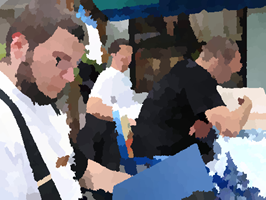
\includegraphics[width=\linewidth]{resources/segm_3_5.png}
			\caption{$\sigma = 3, \tau = 5$}
		\end{subfigure}
		\begin{subfigure}[b]{0.3\linewidth}
			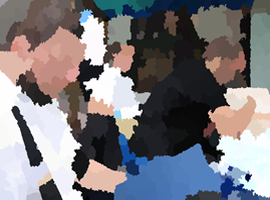
\includegraphics[width=\linewidth]{resources/segm_2_10.png}
			\caption{$\sigma = 2, \tau = 10$}
		\end{subfigure}
		\begin{subfigure}[b]{0.3\linewidth}
			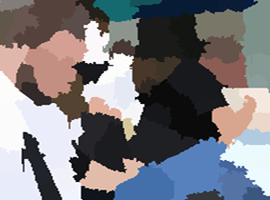
\includegraphics[width=\linewidth]{resources/segm_4_8.png}
			\caption{$\sigma = 4, \tau = 8$}
		\end{subfigure}
		\caption{Segmenting an image with different parameters}
		\label{fig:segmentation}
	\end{figure}
	
	\subsection{Texture analysis}
	The most suitable area for texture analysis was also determined experimentally. As can be observed in figure \ref{fig:texture} the 5x5 window offers a good detection of skin areas while the true positive rate goes down drastically for larger ones. This can be explained by the fact that large patches can cover other surfaces bordering skin such as clothes, eyes, lips, etc.
	
	\begin{figure}[h!]
		\centering
		\begin{subfigure}[b]{0.3\linewidth}
			
\includegraphics[width=\linewidth]{resources/texture_5_5.png}
			\caption{5x5}
		\end{subfigure}
		\begin{subfigure}[b]{0.3\linewidth}
			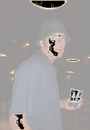
\includegraphics[width=\linewidth]{resources/texture_7_7.png}
			\caption{7x7}
		\end{subfigure}
		\begin{subfigure}[b]{0.3\linewidth}
			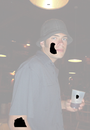
\includegraphics[width=\linewidth]{resources/texture_35_35.png}
			\caption{35x35}
		\end{subfigure}
		\caption{Texture detection with different windows}
		\label{fig:texture}
	\end{figure}
	
	\subsection{Color analysis}
	I tried building color models in RGB, HSV and YCrCb and concluded that Bayesian color analysis obtains roughly the same results regardless of the color space chosen(see table \ref{tab:color_space}). 
	
	For every pixel, I chose the maximum probability on a distance of 4 (similar to the bin size used in \cite{compaq}) on every feature. The threshold value can be used to control the TPR/FPR ratio.
	
	\begin{table}[h!]
		\begin{center}
			\caption{The best performing models for each tested color space}
			\label{tab:color_space}
			\begin{tabular}{c | c|c|c}
				\textbf{Metrics} & \textbf{RGB} & \textbf{YCrCb} & \textbf{HSV} \\
				\hline
				TPR 	  & 0.828 & 0.817 & 0.815 \\
				FPR 	  & 0.227 & 0.216 & 0.209 \\
				Accuracy  & 0.933 & 0.927 & 0.929 \\
				Precision & 0.506 & 0.515 & 0.522 \\
			\end{tabular}
		\end{center}
	\end{table}
	
	\section{Training}
	Training is done separately for each of the main modules: color and texture.
	
	For the training of the color model 2000 images that contain skin and their masks are used, alongside 4000 images that don't contain skin, selected from the Compaq \cite{compaq} dataset.
	
	Texture uses as training data patches from the SFA dataset \cite{sfa}: 3354 skin images of size 5x5 and 5590 non-skin blocks of size 5x5. From these images a total of 8944 textural features are extracted and used to train the SVM.
	
	\section{Evaluation}
	
	\subsection{Dataset}
	The model was evaluated on the Compaq skin database in order to compare it with other approaches from literature. There is a difference however, in the number of images chosen for evaluation. While most references use a ~6000 image set for testing, I used only 150 images due to time constraints.
	
	\subsection{Performance metrics}
	Evaluation is done at the level of each image by comparing every classified pixel with the manually drawn skin map. The results for each image are then averaged to get the final metrics for the data set. The model was evaluated by the following performance indicators: True Positive Rate, False Positive Rate, Accuracy and Precision.
	
	In order to compute those metrics we need to calculate the following values for each image:
	\begin{itemize}
		\item True Positives (TP) - the number of pixels correctly classified as skin
		\item False Positives (FP) - the number of non-skin pixels misclassified as skin
		\item True Negatives (TN) - the number of pixels correctly classified as non-skin
		\item False Negatives (FN) - the number of skin pixels misclassified as non-skin
	\end{itemize}

	The performance metrics can be described as follows:
	\begin{itemize}
		\item True Positive Rate $TPR = TP / (TP + FN)$ - also called Recall, represents the number of skin pixels detected out of the total number of skin pixels in the image
		\item False Positive Rate $FPR = FP / (FP + TN)$ - also called Fall-out, represents the probability of getting a false detection
		\item Accuracy $ ACC = (TP + TN) / (TP + TN + FP + FN) $ - calculates the probability of the correct classification of a pixel 
		\item Precision $ PPV = TP / (TP + FP) $ represents the number of actual skin pixels among all pixels classified as skin
	\end{itemize}

	\subsection{Results}
	Some results of evaluating the proposed model on the Compaq dataset with the parameters set in the previous section and with different threshold values can be seen in table \ref{tab:results}.
	
	\begin{table}[h!]
		\begin{center}
			\caption{Evaluation of the proposed model on the Compaq dataset}
			\label{tab:results}
			\begin{tabular}{c|c|c|c|c}
				\textbf{Threshold} & \textbf{TPR} & \textbf{FPR} & \textbf{ACC} & \textbf{PPV} \\
				\hline
				0.05 & 89.43\% & 31.55\% & 69.84\% & 16.78\% \\
				0.1 & 87.77\% & 21.95\% & 78.69\% & 22.15\% \\
				0.15 & 85.17\% & 16.41\% & 83.69\% & 26.97\% \\
				0.2 & 81.99\% & 12.80\% & 86.84\% & 31.29\% \\
				0.25 & 78.33\% & 10.17\% & 89.06\% & 35.40\% \\
				0.3 & 74.66\% & 8.25\% & 90.61\% & 39.17\% \\
		
			\end{tabular}
		\end{center}
	\end{table}
	
	As seen in the table all runs have a rather low precision, with an average of around 30\%. This is proportional to the number of false positives and is an unresolved problem in skin detection, caused by a large number of skin-like surfaces. This problem can be avoided if detection is done in a controlled environment, like the anchorperson annotation application, but this is not always possible in real world problems.  Most models seen in research have a false positive rate of over 10\%. Papers that I have studied, claiming a smaller false acceptance are evaluated on either unavailable or very small datasets.

	\subsection{Comparison with related work}
	
	In table \ref{tab:results_comparison} there are the results of models found in literature that were evaluated on the same dataset(Compaq). The TPR and FPR are the most common metrics used for skin model evaluation.
	
	\begin{table}[h!]
		\begin{center}
			\caption{Comparison of the proposed model with related work}
			\label{tab:results_comparison}
			\begin{tabular}{c|c|c}
				\textbf{Model} & \textbf{TPR} & \textbf{FPR} \\
				\hline
				Proposed model & 85.17\% & 16.41\% \\
				SPM model (Jones and Rehg \cite{compaq}) & 90\% & 14.2\% \\
				Mixture of Gaussians (Jones and Rehg \cite{compaq}) & 80\% & 9.5\% \\
				Single Gaussian CbCr (Lee and Yoo \cite{gaussian_applied}) & 90\% & 33.3\% \\
				Gaussian Mixture IQ (Lee and Yoo \cite{gaussian_applied}) & 90\% & 30\% \\
				YI'Q' thresholding (Brand and Mason \cite{i_threshold_applied}) & 94.7\% & 30.2\% \\
				Elliptical boundary model (Lee and Yoo \cite{gaussian_applied}) &
				90\% & 23.3\% \\
				Segmentation and SPM (Poudel and Zhang \cite{superpixels_applied_2}) & 91.17\% & 13.12\% \\
				
			\end{tabular}
		\end{center}
	\end{table}
	
	My model obtains comparable results to state of the art approaches, even outperforming the thresholding approaches, but a bit worse than the best models available. Some factors which I think contributed to underperforming are image resizing and using a smaller subset for evaluation. 
	
	My algorithm resizes every image to increase performance. However, this means that it must use a smaller window for texture analysis which might not be enough to get relevant textural features.
	
	I have only used a subset of 150 images, 50 containing patches of skin, for evaluation due to its computation time, while most models use around 6000 images (2000 skin and 4000 non-skin). The images selected for my model could have been not very representative for the dataset. Furthermore, when experimenting with increasing the testing set I have noticed improvements in performance. This suggests that on a dataset similar to that used by compared models, 2000 skin and 4000 non-skin images, performance may increase considerably.
	
	\newpage
	\subsection{Detection examples}
	\begin{figure}[h!]
		\centering
		\begin{subfigure}[b]{0.4\linewidth}
			\includegraphics[width=\linewidth]{example_runs/1_in.png}
		\end{subfigure}
		\begin{subfigure}[b]{0.4\linewidth}
			\includegraphics[width=\linewidth]{example_runs/1_out.png}
		\end{subfigure}
		
		
		\begin{subfigure}[b]{0.4\linewidth}
			\includegraphics[width=\linewidth]{example_runs/2_in.png}
		\end{subfigure}
		\begin{subfigure}[b]{0.4\linewidth}
			\includegraphics[width=\linewidth]{example_runs/2_out.png}
		\end{subfigure}
		
		\begin{subfigure}[b]{0.4\linewidth}
			\includegraphics[width=\linewidth]{example_runs/3_in.png}
		\end{subfigure}
		\begin{subfigure}[b]{0.4\linewidth}
			\includegraphics[width=\linewidth]{example_runs/3_out.png}
		\end{subfigure}
		
		\caption{Some detection examples. Skin is marked with a black mask.}
		\label{fig:example_detection}
	\end{figure}
	
	\chapter{Application development}
	In this chapter all details related to the application implemented for the model proposed in the previous chapter are presented. The first section reviews the libraries and frameworks used in the project. The following section is focused on design and contains a breakdown of every module and an overview of the main use cases. The last section presents the functionalities of the application in a user friendly way.
	
	\section{Technologies used}
	
	\subsection{General}
	The application is implemented entirely in the Python programming language, which is a high-level language with dynamic types. Furthermore it has a rich ecosystem with mature frameworks relevant to machine learning and image processing. Even though it does not offer a performance as good as lower level languages, Python shines through its simplicity and numerous libraries.
	
	For simple use of tuples the python namedtuple module was used. This is basically a way to assign names to tuple fields. The reason for using tuples is to set dictionary keys, which are required to be immutable values. The two named tuples used in the application are pixel position (x, y components) and color features. The advantage over using custom classes as keys can be found in the performance difference.
	
	Model serialization and deserialization is done using the python pickle module. This is a very simple yet efficient serializer, suited for tasks that don't require complex serialization logic.
	
	\subsection{Image processing}
	OpenCV \cite{opencv} is a very popular library for image manipulation available for Python and C++. In this project OpenCV was used for some trivial image processing tasks such as: reading and writing images to a folder, conversions between color spaces and applying masks to images. 
	
	OpenCV manipulates all images as NumPy \cite{numpy} arrays and this convention was kept throughout the rest of the code. NumPy is a very powerful array manipulation library used in scientific computing projects, offering a similar performance to Matlab. NumPy's speed is attributed to having many of its operations, such as loops, implemented in C.
	
	\subsection{Texture analysis}
	For the quick evaluation of Haralick's feature the Mahotas \cite{mahotas} library is used. It is a computer vision library which offers a Python interface, appropriate for fast development, but the underlying implementation is in C++, mainly for performance. While not as popular as OpenCV, it contains some algorithms that the other library lacks, such as Haralick feature extraction. Like most Python image processing libraries, Mahotas operates on Numpy array, which matches the project's image handling standard.
	
	The machine learning classifier employed by the model was a Support Vector Machine taken from the sk\_learn framework \cite{scikit-learn}. This library offers simple and efficient data analysis tools focused on accessibility and was designed to work well with other Python packages such as NumPy. It's name comes from "SciPy Toolkit", meaning it is an extension of SciPy, a popular Python library used for scientific computing. Similarly to other high-performance modules, sk\_learn has an underlying C implementation. The chosen classifier for this project is the LinearSVC, which uses a linear kernel due to its speed.
	
	\subsection{GUI}
	The Graphical Interface is implemented using the TkInter framework \cite{tkinter}. This is the most used GUI in Python and with the most available resources. Another advantage of this framework is the simplicity of building interfaces. Every window can be defined in a class and then they can be composed in a tree-like structure and reused in multiple parts of the application. It offers a simple approach to widget positioning using grids. TkInter also provides portability for the main Operating Systems and comes with a native look for each.
	
	In order to get a responsive UI the threading and multiprocessing modules are used. Whenever a new process (like detection or evaluation) is started a new process is created for it. The application also creates a new thread that communicates with that process and updates the UI widgets.
	
	\clearpage
	\section{Implementation and design}
	
	\subsection{Architecture}
	
	The application is made up out of five main modules, pictured in figure \ref{fig:main_modules}: segmentation, $color\_analysis$, $texture\_analysis$, evaluator and $application\_gui$. The first three provide the basic image processing operations, the evaluator provides an interface for detection and performance measurements while the top module offers a visual interface for user convenience. I will present them in detail in separate sections.
	
	\begin{figure}[h!]
		\centering
		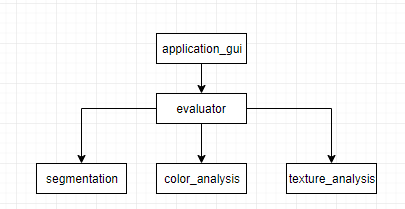
\includegraphics[]{design/main_modules.png}
		\caption{Main modules}
		\label{fig:main_modules}
	\end{figure}

	\subsubsection{The image segmentation module}
	An overview of this module can be seen in figure \ref{fig:image_segmentation}. The segmentation functionality is provided by the QuickshiftSegmentation class, which exposes two public methods, apply(image) and $get\_superpixels(image)$, and takes the sigma and tau parameters in the constructor. The first method applies Quick shift segmentation on the image and returns an image where regions are visible, being colored with the same value as the root pixel. The second method returns a map containing all identified regions. The keys are roots pixels and the values their corresponding superpixels. 
	
	Regions are represented by the Superpixel class whose fields are: the initial image, position of the root pixel and a list of positions of all corresponding pixels.
	
	The Distances class encapsulates some methods used by the segmentation algorithm to calculate pixel and feature distances.
	
	\begin{figure}[h!]
		\centering
		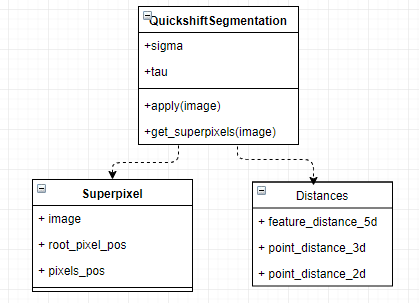
\includegraphics[]{design/image_segmentation.png}
		\caption{Image segmentation module}
		\label{fig:image_segmentation}
	\end{figure}

	\subsubsection{The color detection module}
	This module can be divided into two submodules: training, figure \ref{fig:color_train}, and detection, figure \ref{fig:color_detect}.
	
	In order to train a color detection model you must call the $train\_spm\_model$ static method which takes a SPMTrainConfiguration object. The configurable fields are the database (SFA or Compaq), the color space (RGB, HSV, YCrCb) and paths for resources. 
	
	Depending on the value of the database parameter the trainer creates either a SfaComponentExtractor or a CompaqComponentExtractor. Both of these classes provide a method $extract\_components$ that returns a BayesSPMComponents object, which encapsulates: the number of skin and non-skin pixels, a map with the number of apparitions for each pixel and a map with the number of apparitions as skin.
	
	The resulting model, a SPMModel object, is serialized into a file. It contains the selected color space and the components extracted on the previous step.
	
	\begin{figure}[h!]
		\centering
		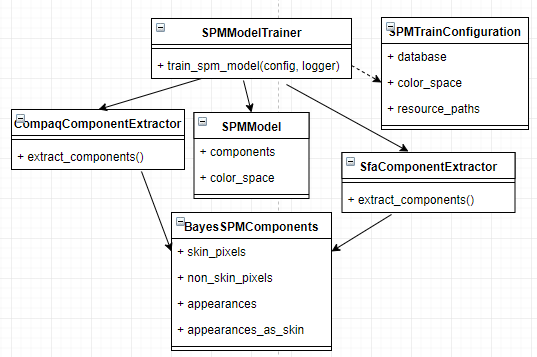
\includegraphics[]{design/color_train.png}
		\caption{Color detector training submodule}
		\label{fig:color_train}
	\end{figure}
	
	Depending on the input parameters the SPMDetectorFactory provides one of the following detectors: SimpleDetector, NeighborDetector or AverageOnSuperpixelDetector. The first one is the simplest approach as it calculates a probability for each pixel independently. The second, takes into account an area around each pixel. This simulates the histogram based approach with the difference that the considered pixel is always at the center of the area. The last detector calculates the average probability of a given superpixel.
	
	All detectors use the methods defined in ProbabilityCalculator through an intermediary layer. This proxy, CachedProbabilityCalculator, was created to speedup operations by caching probabilities. The need for memorizing these values arose from the fact that images usually contain a small subset of pixel values duplicated many times.
	
	\begin{figure}[h!]
		\centering
		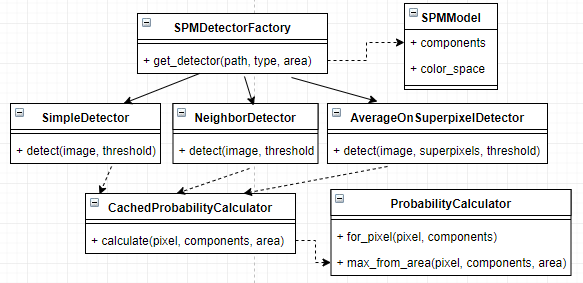
\includegraphics[]{design/color_detect.png}
		\caption{Color detection submodule}
		\label{fig:color_detect}
	\end{figure}
	
	\subsubsection{The texture analysis module}
	Similarly to the previous module, texture analysis can be divided into two submodules, one for training, figure \ref{fig:texture_train}, and one for detection, figure \ref{fig:texture_detect}.
	
	The model used in skin texture detection, TextureModel, has an attribute for extracting textural features from images (feature\_extractor), one for classifying those values (classifier), and label for interpreting the classifier's results (skin\_label). This model is trained by a HaralickModelTrainer which gets its parameters from a TextureTrainConfig object.
	
	In this project there is only one implemented model based on Haralick's features but the design allows incorporating other methods. The HaralickModel extends the basic TextureModel and overrides the feature extraction method. It is trained by a HaralickModelTrainer which injects a feature extraction object and a classifier into the model. 
	
	The selected feature extractor is a HaralickFeatureExtractor, which encapsulates Haralick's method taken from the mahotas library. The chosen classifier is returned by SvmClassifier's static method (train\_svm\_classifier) which trains a Support Vector Machine model using the sk\_learn library. The model trainer is also responsible for selecting a method of preparing the input data, in this case using the TrainDataPreparer class, which computes Haralick's features and appends the corresponding label.
	
	\begin{figure}[h!]
		\centering
		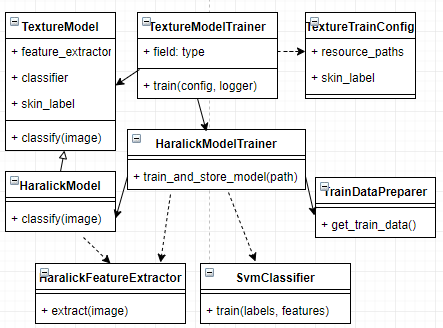
\includegraphics[]{design/texture_train.png}
		\caption{Texture detector trainer submodule}
		\label{fig:texture_train}
	\end{figure}

	There are two types of detectors available. The GridDetector slides a window over the image and classifies each of those blocks. The PerPixelDetector is a more precise approach because it builds a window around each pixel in the image and only marks the center pixel. Although the second approach gains a noticeable increase in precision, it is much slower than the first.

	\begin{figure}[h!]
		\centering
		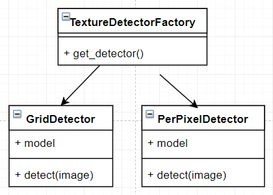
\includegraphics[]{design/texture_detect.png}
		\caption{Texture analysis submodule}
		\label{fig:texture_detect}
	\end{figure}
	
	\subsubsection{The evaluator module}
	
	The evaluator module has a simple structure, as seen in figure \ref{fig:evaluator}. The Evaluator class contains methods for evaluating a model(run\_simulation) and for applying it to an image(run\_detection). It takes as input a RunConfiguration object which contains informations about the desired skin and texture models and segmentation parameters.
	
	In order to evaluate the model some quality measures are applied for each analyzed picture. These measurements include the number of true positives, false positives, true negatives, false negatives and are implemented by the Stats class. The results are logged and also saved to a file in the csv (Comma-separated Values) format for later analysis.
	
	\begin{figure}[h!]
		\centering
		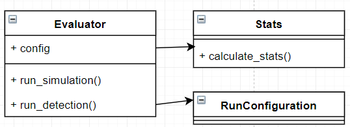
\includegraphics[]{design/evaluator.png}
		\caption{The evaluator module}
		\label{fig:evaluator}
	\end{figure}
	
	\subsubsection{User interface}
	
	The user interface was build using the TkInter library. This framework was designed to create modular applications. Consequently every window can be composed out of multiple frames, which are reusable components. The main views used in the application are visible in figure \ref{fig:gui}. The various configuration frames were left out of the diagram to avoid clutter.
	
	MainView is a tab-view component which is provides links to the application's main windows: color model training, texture model training, model evaluation, detection of a picture.
	
	Every component has a ProcessControlFrame which contains a FeedbackFrame and some buttons for starting and stopping operations. When the user presses the 'Start' button a new process is launched which performs the request and logs results into a queue. A monitoring thread reads that from the queue and passes it to the FeedbackFrame for displaying it on the screen. This approach allows the user to follow the application's progress while keeping the user interface decoupled from the algorithms.
	
	The detection view also contains an ImageDisplayFrame, which displays the input and the resulting image.
	
	\begin{figure}[h!]
		\centering
		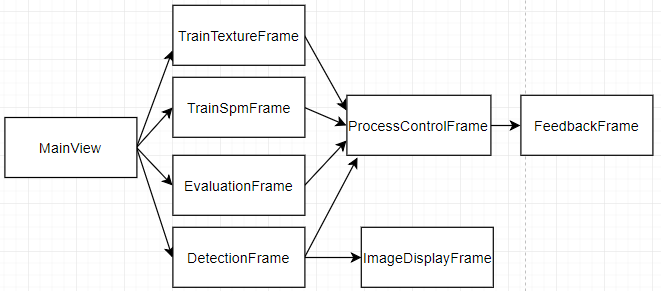
\includegraphics[]{design/gui.png}
		\caption{The user interface module}
		\label{fig:gui}
	\end{figure}
	
	\clearpage
	\subsection{Use cases}
	The main use cases are illustrated in figure \ref{fig:use_cases}. These are the hybrid model training, which includes the color and texture model training, model evaluation and detection on particular images. In order to evaluate a model the user should train it first. Also, it is recommended to evaluate the model before using it for other tasks.
	
	All use cases allow the user to set various parameters and resource paths. Resources include: training, evaluation and testing images, selected models.
	
	\begin{figure}[h!]
		\centering
		\includegraphics[]{design/use_cases.png}
		\caption{The application use cases}
		\label{fig:use_cases}
	\end{figure}

	\clearpage
	\subsection{Sequence diagrams}
	
	\subsubsection{Image skin detection}
	This section illustrates the use case of skin detection for an image. The sequence diagram associated with this flow can be seen below, in figure \ref{fig:detection_sequence}. 
	
	First, the user uploads the desired model, selects the image on which detection will be run and sets some tweaking parameters. After pressing start, a new evaluator is created in a separate process and a message is dispatched with the desired image. The evaluator calls three components: \textbf{segmentation}, represented by the quick shift algorithm, which returns a list of superpixels, \textbf{color analysis}, which uses SPM techniques on the superpixels from the previous call, and \textbf{texture detection}, which returns a texture mask for the initial image. The evaluator then combines the resulting masks and sends a message back to the GUI (DetectionWindow) which displays the results.
	
	\begin{figure}[h!]
		\centering
		\includegraphics[]{design/sequence_detection.png}
		\caption{Skin detection sequence diagram}
		\label{fig:detection_sequence}
	\end{figure}

	The image evaluation sequence diagram is omitted because it is very similar to the detection process applied to multiple images. The main difference is that after detection, a comparison is made between the given mask and the model's result.
	
	\clearpage
	\subsubsection{Texture model trainer}
	The sequence diagram for the texture model training use case can be seen in figure \ref{fig:texture_sequence}. 
	
	The user has to select folder for model training, one for images of skin and one for images not containing skin, and to provide a path where to store the resulting model. The application creates a new process responsible for training the texture model and dispatches a request to it with the training data location.
	
	The TextureModelTrainer component requests a set of features and labels from the TrainDataPreparer. The latter reads the training data and loops over each image to get its features from the  feature extraction component. After the trainer receives all textural features it uses them to train a Support Vector Machine. The resulting model is stored to a configured location and the GUI receives a message indicating the process has finished, which is then displayed on the screen.
	
	\begin{figure}[h!]
		\centering
		\includegraphics[]{design/sequence_texture_train.png}
		\caption{Texture model training sequence diagram}
		\label{fig:texture_sequence}
	\end{figure}
	
	The sequence diagram of training the color model is not presented as it resembles the one illustrated in this section.
	
	\clearpage
	\section{User manual}
	\subsection{Introduction}
	The goal of this application is to provide an easy-to-use and highly-configurable interface for training and evaluating skin detection models that share a core structure of image segmentation, color and texture analysis. The user can also test the created models on individual images. As the number of parameters for each task can be overwhelming the user can opt to use the default values that have already been set in each field.
	
	The application does all computing intensive tasks in separate processes. This means the user can perform multiple operations, e.g. evaluate a model on the validation dataset and perform some single image detections on the same model, at the same time.
	
	The application has 4 main windows accessible through a tab-view set in the top-left corner. The windows, detailed in the following sections, are the Evaluator, Train SPM, Train texture and Detection windows.
	
	\begin{figure}[h]
		\centering
		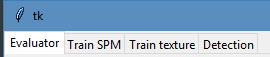
\includegraphics{manual/tab_view.png}
		\caption{The tab-view main menu}
	\end{figure}
	
	\subsection{Detection view}
	This view allows the user to test the model on individual images and get visual feedback. The resulting image will be displayed on the screen with a black mask that marks the identified pixels. This window provides a quick way to evaluate a model or to make a demonstration.
	
	If you want to apply the model to a single image you must specify the detection parameters, or go with the default ones, provide a path to the input image (bottom frame on the left side of the screen) and click ‘Start experiment’. The initial image and the result will be displayed on the frames on the right side of the screen. The other configuration frames are explained in detail in section \ref{configuration_frames}. 
	
	On the middle of the screen, below the buttons for controlling the experiment, you will see updates of the detection process. A progress bar will follow the time consuming operations: segmentation, color and texture analysis.
	
	\begin{figure}[h!]
		\centering
		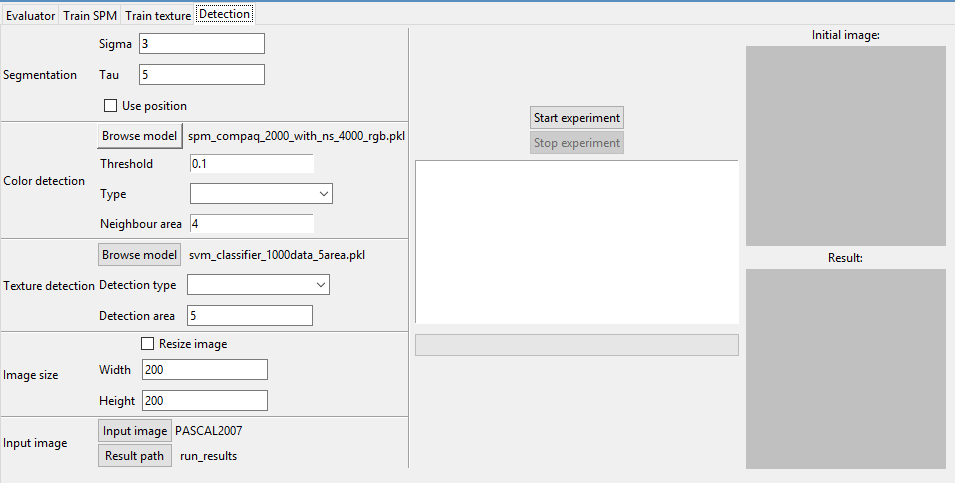
\includegraphics[width=\linewidth]{manual/detection_view.png}
		\caption{Detection view}
	\end{figure}
	
	\subsection{Evaluator view}
	
	This screen allows the user to evaluate the performance of the final model and follow the progress in real time. The selected model can be configured in various ways which will be presented in detail in the common configurations section.
	
	\begin{figure}[h!]
		\centering
		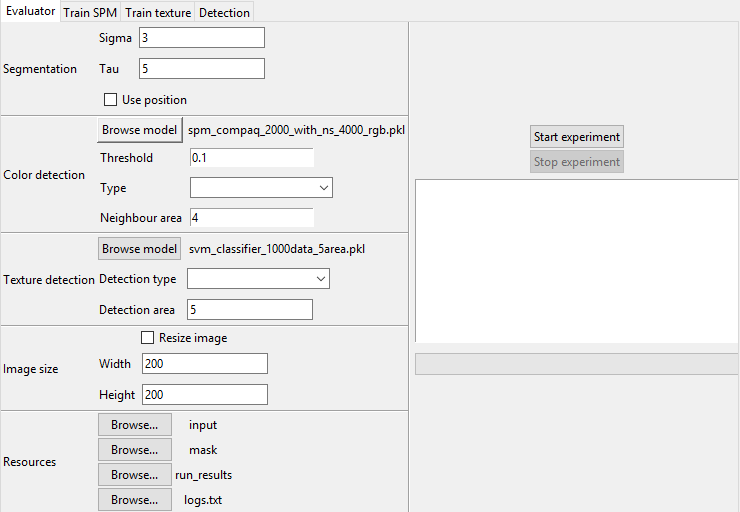
\includegraphics[width=\linewidth]{manual/evaluator_view.png}
		\caption{Evaluator view}
	\end{figure}
	
	The application applies the selected model to images from the provided folders. Input images can have any size and name. Masks should have the same size and name as their corresponding input and should mark skin pixels in black (0, 0, 0). The paths where execution logs and run results are stored are also customizable.
	
	To begin evaluation you must press ‘Start experiment’. The frame below the button displays information about the currently processed picture, the operation in progress and evaluation results. 
	
	A progress bar will indicate the status of each action applied to the image. The main actions are, in order: image segmentation (consisting of density computation, neighbor linking and superpixel extraction), color detection (Bayes SPM), texture analysis (Haralick feature, combination of results and metrics calculation. Images obtained for each step (color, texture and their combination) are all saved in the results folder, to facilitate the identification of cases for which the model does not perform as expected.
	
	After each picture is analyzed by the model, the performance metrics(true positive rate, false positive rate, true negative rate, false negative rate, accuracy, precision and recall) are displayed on the screen and saved to a file.
	The application builds a csv file containing metrics from each processed picture, that can be used to obtain overall results. A dump of the initial configuration is done in the file $initial\_config.txt$ for documentation purposes.
	
	\subsection{Color model training view}
	This window is used to train a Bayesian color detection model. You can select a color space, the path to input data (a folder which should contain the following subfolders: train\textunderscore images – images containing skin, train\textunderscore images\textunderscore ns – images not containing skin, train\textunderscore masks – masks for images containing skin), the name of the model and the path to the folder where it will be stored. 
	
	The model, consisting of a map of pixel values and their count, is stored alongside color space meta data in a .pkl file, which can be later imported by the application for evaluation.
	
	Similarly to the other views, to start training the model you must press the ‘Start experiment’ button. In the frame below you will see status updates for loading images and extracting features from them as well as a progress bar for each operation.
	
	\begin{figure}[h!]
		\centering
		\includegraphics[width=\linewidth]{manual/color_model_train_view.png}
		\caption{Color model training view}
	\end{figure}
	
	\subsection{Texture model training view}
	The process of training a texture detector is simple. You must select folders with images of skin, images not containing skin and a path to store the resulting model.
	
	After pressing ‘Start experiment’ the training begins and you will see updates for feature extraction and machine learning analysis. First, the process builds a list of features and tags (skin/non-skin) from positive and negative images. Then, those features are analyzed by a SVM algorithm and the resulting model is stored in a .pkl file. That file contains the SVM's result, the serialized function for feature extraction and the tag used to identify skin texture.
	
	\begin{figure}[h!]
		\centering
		\includegraphics[width=\linewidth]{manual/texture_model_train_view.png}
		\caption{Texture model training view}
	\end{figure}
	
	\clearpage
	\subsection{Common configuration frames} \label{configuration_frames}
	Some or all of these model configuration frames are present on multiple views. For this reason they are presented in a single section.
	
	\subsubsection{Segmentation}
	
	\begin{wrapfigure}{r}{0.5\textwidth}
		\begin{center}
			\includegraphics[]{manual/segmentation_frame.png}
		\end{center}
		\caption{Segmentation configuration frame}
	\end{wrapfigure}
	
	The segmentation frame is used for tuning the parameters of the quickshift image segmentation algorithm. 
	
	Sigma controls the shape of the superpixels and Tau the size, and you can set them by typing in their adjacent textboxes. 
	
	The ‘Use position’ checkbox indicates whether the algorithm should consider pixel position in image as a feature for density calculation. If this box remains unchecked the density function will consider only the color space information.
	
	\subsubsection{Color detection}
	
	\begin{wrapfigure}{r}{0.6\textwidth}
		\begin{center}
			\includegraphics[]{manual/color_detection_frame.png}
		\end{center}
		\caption{Color detection configuration frame}
	\end{wrapfigure}
	
	This frame provides configurations for the color detection module.
	
	The SPM model is a pickle (.pkl) file generated from the Train SPM view. This indicates which color model should be selected for Bayesian probability calculations. 
	
	The detection threshold is a value between 0 and 1 which indicates at what probability to start considering pixels as skin. Consequently all pixels or clusters for which the model calculates a probability higher than the threshold are classified as skin pixels.
	
	The type of the SPM classifier can be selected from the 'Type' dropdown widget.
	There are two types: average probability over superpixel and probability for the root of the superpixel. This affects how the probabilities are calculated for the regions identified during segmentation.
	
	The neighbor area represents the considered neighbors during the computation of a pixel's skin probability. The final probability is taken as the maximum value obtained by exploring the color space in every direction on a distance limited by this parameter. 
	
	\subsubsection{Texture detection}
	\begin{wrapfigure}{r}{0.6\textwidth}
		\begin{center}
			\includegraphics[]{manual/texture_detection_frame.png}
		\end{center}
		\caption{Texture detection configuration frame}
	\end{wrapfigure}
	
	By clicking on the ‘Browse model’ button you can select the texture analysis model, which is a SVM classifier stored as a pickle file. This model is generated from the 'Train texture' window.
	
	From the ‘Detection type’ dropdown you can select the texture detection strategy:
	\begin{itemize}
		\item Window scan, which slides a window over the image, is fast but produces jagged edges
		\item Around each pixel, which builds a window around each pixel, is slow but obtains smoother results
	\end{itemize}
	
	The size of these windows is set from the ‘Detection area’ text field.
	
	\subsubsection{Resize options}
	
	\begin{wrapfigure}{r}{0.5\textwidth}
		\begin{center}
			\includegraphics[]{manual/resize_frame.png}
		\end{center}
		\caption{Size configuration frame}
	\end{wrapfigure}
	
	If you wish to resize the image you must check the ‘Resize image’ box and then specify the given parameters. This is usually done for increasing computation speed.
	
	If you do not check the box then the image will be processed in its original size.
	
	\subsection{User Feedback}
	
	The feedback view can be seen in figure \ref{feedback_view} and is present on each window. It is a text box that displays feedback from the application. It also contains the 'Start experiment' and 'Stop experiment' button which control the process associated with the view: detection, evaluation or training.
	
	On the bottom of the frame there is a progress bar that keeps track of the current operation, for example: density calculation, superpixel extraction, SPM detection etc. That operation is also displayed in the label underneath the progress bar.
	
	
	\begin{figure}[h!]
		\centering
		\includegraphics[]{manual/feedback_view.png}
		\caption{Feedback view}
		\label{feedback_view}
	\end{figure}

	\chapter{Conclusions}
	This chapter gives contains remarks on the current state of research in skin detection and what could be improved. It also presents the conclusions of the experiment described in this paper and offers some directions of improvement.
	
	\section{State of research}
	Skin detection has been a topic of interest in research for many years and it is still active. Color analysis, being the fastest technique and the one offering the best recall is the base of almost skin detector in literature. Its drawback, the rather high false detection rate, is usually ignored or mitigated with either a texture detector or segmentation pre-processing step. I haven't encountered a model that uses both, possibly due to the trade-off in computation time.
	
	A pressing issue in the field is the lack of a modern, large and diverse dataset to be used as a standard for evaluating models. The Compaq database, which is currently the most popular, was composed in the 90s and most images have a rather low quality. The SFA and other similar face-oriented databases, contain humans in a controlled environment, usually in the same position, with only the face and sometimes hands as skin regions. A lot of papers claiming to have greatly reduced the false acceptance rate use either very small or self-built unavailable datasets. This is the main reasons that make it difficult to accurately compare and evaluate skin detection models.
	
	\section{Proposed model's results}
	
	The proposed model obtains similar but slightly worse results than the state-of-the-art techniques. Consequently, it has not achieved its goal of considerably reducing the large false positive rate currently associated with skin detection models. The reasons for this could be the resizing step which forces the selection of a smaller texture detection window or the use of a small dataset for evaluation in comparison to other models. Both of these compromises have been taken due to time constraints. This indicates the proposed model is unfit for real-time detection tasks but could be a valid approach for data mining processes.
	
	\section{Future developments}
	A big issue in the current form of the model is the computation time, which forced me to take some decision that might have impacted classification performance. Consequently this would be the top candidate for optimization. Some solutions in this direction are implementing the image processing algorithms on the GPU (an example for Quick shift was provided by Fulkerson \cite{quickshift_gpu}) and take advantage of multithreading whenever possible (for example during evaluation).
	
	Another area of improvement is in texture detection. Upon analysis of the visual feedback, the current texture model does not provide an improvement as large as expected. Some alternative texture analysis techniques such as Gabor filters could be tested.
	
	Even though I tried to cover the most important directions of skin analysis, there are some aspects I didn't consider. For example, the addition of a shape based model could help further reduce false acceptance rate.
	
	\newpage
	\bibliographystyle{apa}
	\bibliography{references}
\end{document}